% Lines that start with a % are comments and are not included when the LaTeX file is converted to a pdf

% Set up the document class - this can be changed if a different format is required 
\documentclass[11pt,a4paper,twoside]{article}

% Include packages that contain additional features, for example including special mathematical characters and images in your document
\usepackage{amssymb,amsmath,graphicx}
\usepackage[T1]{fontenc} 
\usepackage[utf8]{inputenc}   % here are our umlauts...
\usepackage{graphicx} % ...and our graphics
\usepackage{listings}
\usepackage{bold-extra}
\usepackage[plainpages=false, pdfpagelabels, colorlinks=true, breaklinks=true, linkcolor=black, menucolor=black, urlcolor=black, citecolor=black]{hyperref}
\usepackage[font=sf, labelfont={sf,bf}, margin=1cm]{caption}
\usepackage[b]{esvect}
% Long equations
\usepackage{breqn} 
%include pdfs
\usepackage{pdfpages}
\usepackage{hyperref}
\usepackage{epstopdf}
%\usepackage{fullpage}
\usepackage{placeins}
\usepackage{pdfpages}


% The beginning of the document...
\begin{document}
\renewcommand\thesubsection{\alph{subsection})}

% configure standard code listings:
\lstset {
language = bash,
	breaklines = true,
	breakatwhitespace = true
}

% Please change the following accordingly...
\centerline{\LARGE \textbf{Artificial Intelligence - Exercise Sheet 7}}\vspace{0.5em}
\centerline{\large by Lucas-Raphael Müller}\vspace{2em}


\section{Types of Learning}
\paragraph{Supervised Learning} is the type of learning where training data comes along with target images. Easy examples are handwritten digits, such as the MNIST dataset. Labeled data allows for computing a loss.
\paragraph{Unsupervised Learning} does not allow for the computation of a loss, since input data is unlabeled, i.e. without ground truth.
The task is to infer similarities among input data.  
An example would be facial recognition without knowing who is on which picture.
\paragraph{Semi-supervised Learning} is a mixture of super- and unsupervised learning, where some input data comes labeled, some not.
\paragraph{Reinforcement Learning} features a reward, which has to be maximised (minimised) by the algorithm with a not defined action within a defined set of possible actions (e.g. put a coin in column 1-7).
For example, a connect4 session where player A won, could be rewarded with 1, a session which has been lost with -1 and a draw with 0.
A probably faster converging reward function in this case would be 100 for a session which has been won, 10 for 3 coins in a row, 1 for 2 in a row.

\section{Learning as an Optimisation Problem}
With
\begin{align}
	y &= f(x,W) \\
	r_i = e_i &= f(x_i,W) - y_i,
\end{align}
\paragraph{Optimisation Problem} We can use
\begin{align}
	\min\limits_W F(W,{(x_i,y_i)}_{i=1}^m)
\end{align}
with
\begin{align}
	F(e_i) = \sum\limits_i r_i^2,
\end{align}
which is indeed least-squares optimisation.

\paragraph{Finding a solution} by differentiation
\begin{align}
	-2\sum _{i}r_{i}{\frac  {\partial f(x_{i},{\boldsymbol  W })}{\partial W _{j}}}=0,\ j=1,\ldots ,m,
\end{align}
for parameters $W_j$.

\paragraph{NN Triple Junction}
For the triple junction we need at least 3 linear functions.
I would argue at least 2 layers, one to divide in two subsets, and one additional do divide into the third?

\section{Implementing a simple Classification Example}
I converted the target into one-hot vectors since neural networks tend to be more efficient when one encodes each output neuron to one output.
Mathematically one could also encode two multiple labels into one output neuron.
However then I ran into some difficulties with decision boundary visulisation.
\paragraph{Network Architecture} I used a deeper but with fewer neurons per layer network in the first case, and a two layer network in the latter.
The former features tanh activation function, the latter Relu.
Since I converted into one-hot, a softmax is applied in the last step in order to get probabilities in the range from 0 to 1.

\paragraph{Loss Function} I used MultiLabelSoftMarginloss which should be the apropriate for multilabel classification.
If I were not to convert to one-hot vector, MSE-loss would be probably possible as well.

\paragraph{Optimiser} SGD which is apropriate for mini-batch. However since I used my own data loader and I ran into time issues what I did is not really mini-batch... .
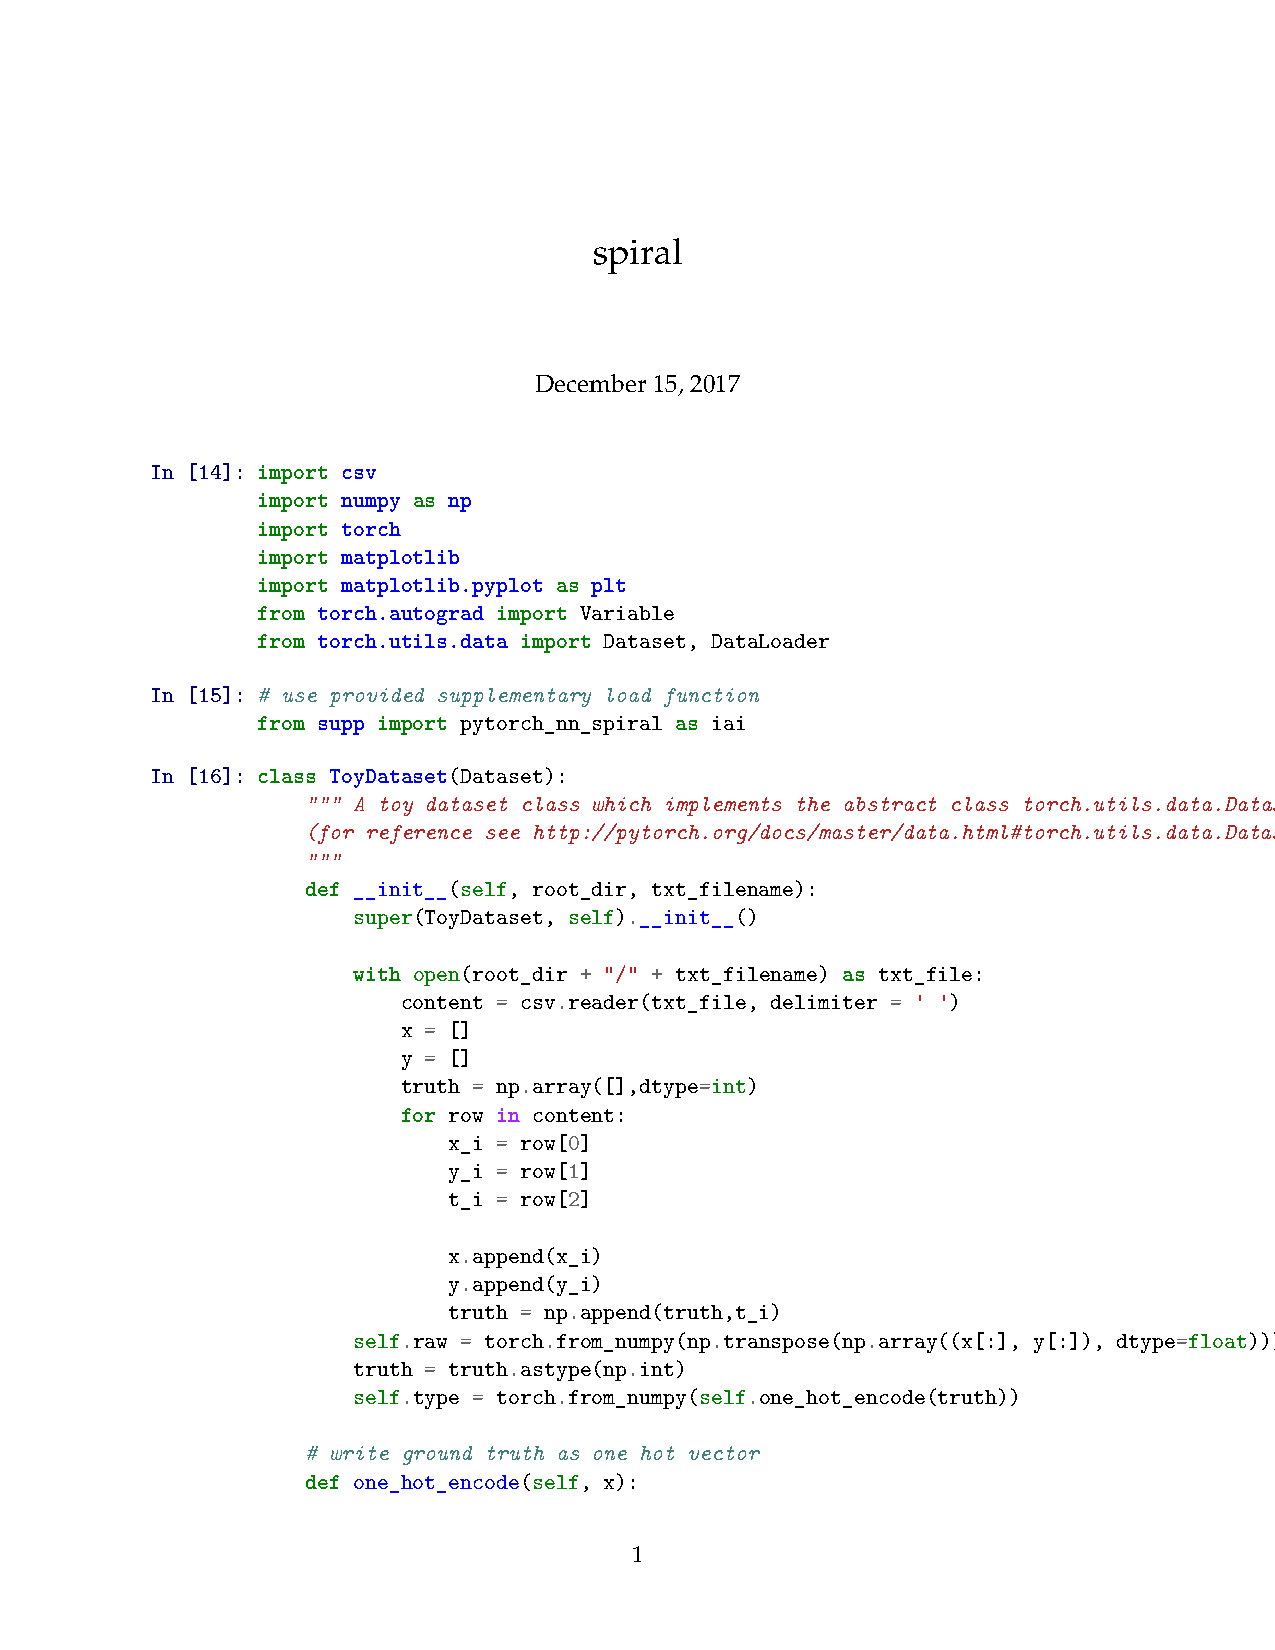
\includepdf[pages=-]{spiral.pdf}
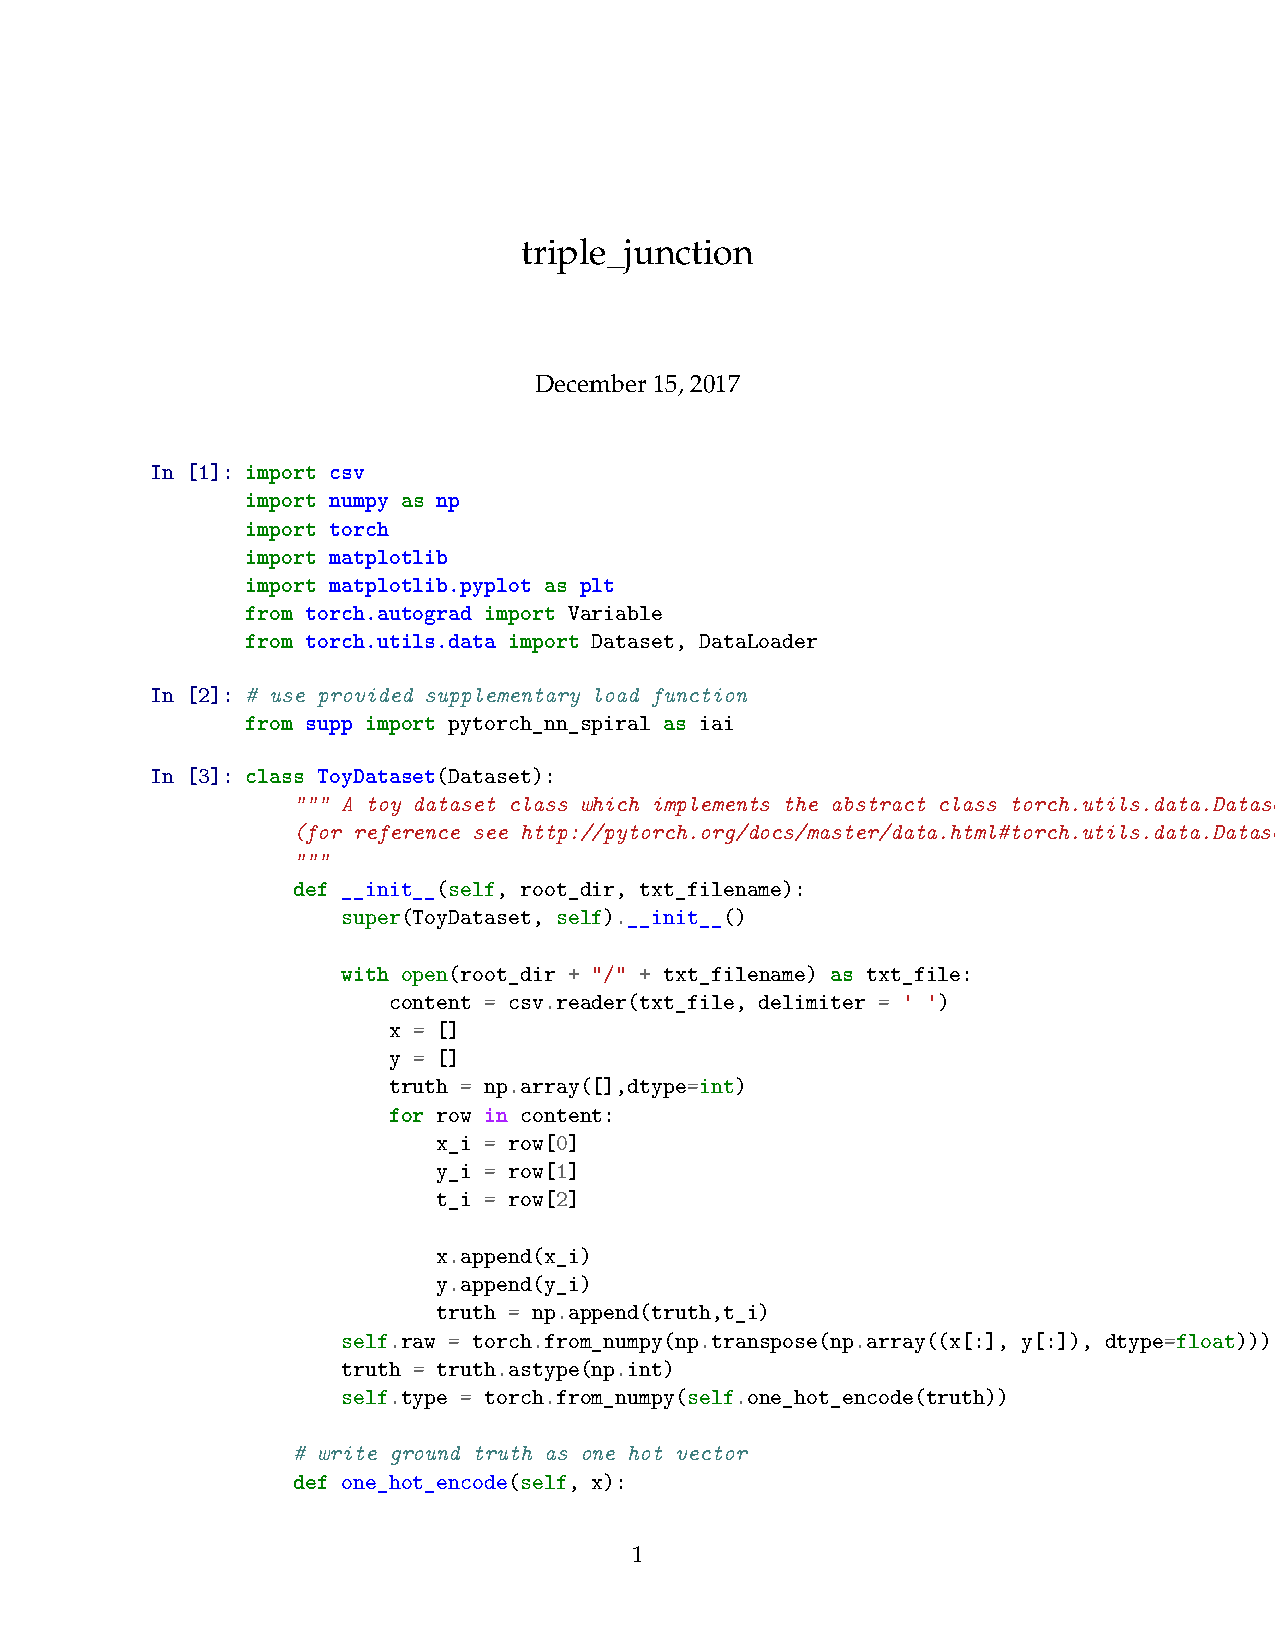
\includepdf[pages=-]{triple_junction.pdf}

\section{CNN for MNIST}
Confusion matrix on test set.
\begin{figure}[!h]
	\centering
	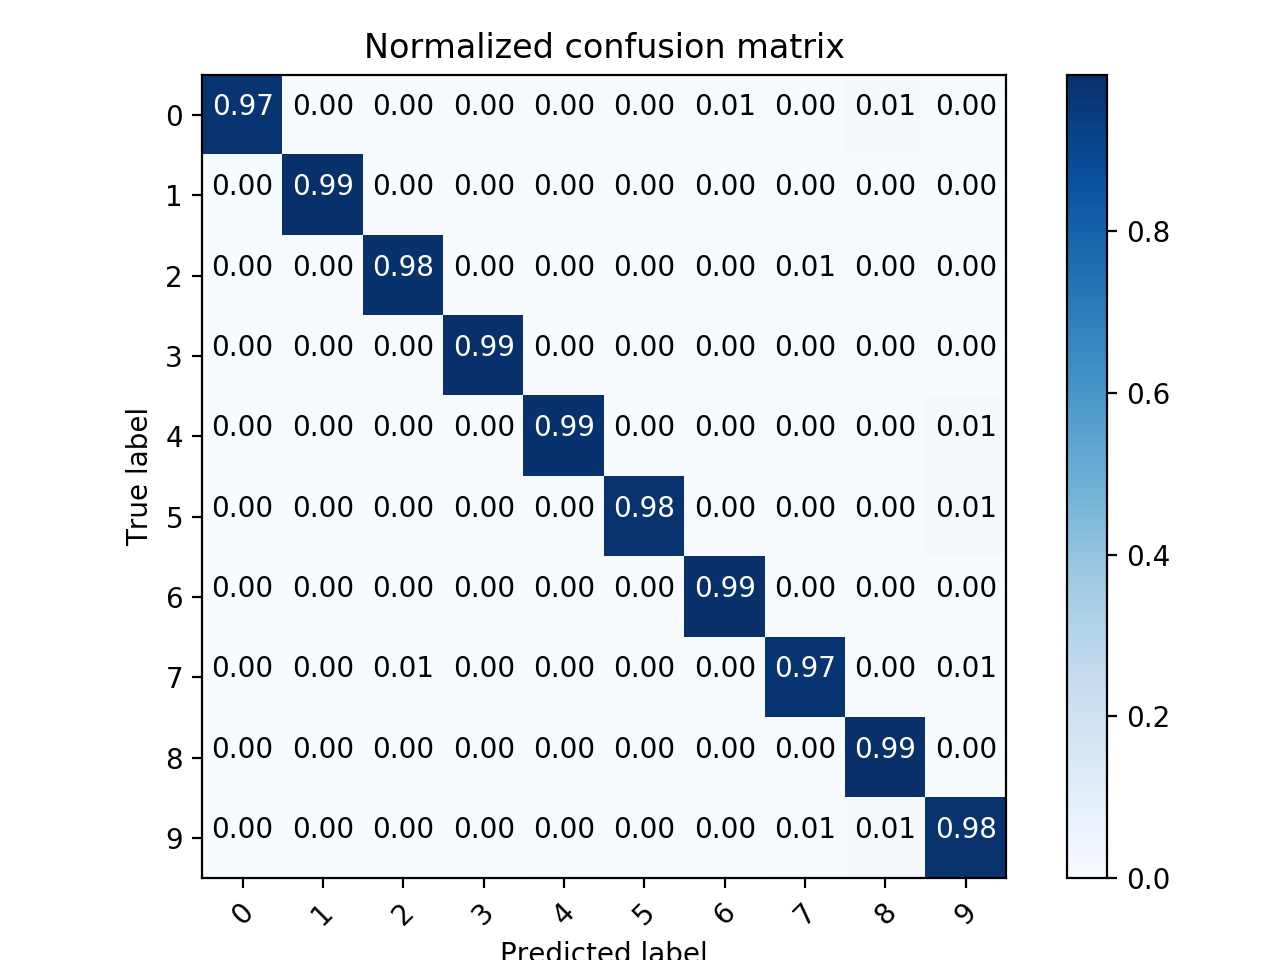
\includegraphics[width=.8\textwidth]{confusionMat}
	% \caption{$jkl$ }
	\label{gauss1}
\end{figure}


\FloatBarrier

\newpage
\section{Appendix: Python Source Code}
\label{sec:app}

\subsection{CNN Code}
\lstinputlisting[language=Python]{cnn.py}

\end{document}
